\chapter*{Discussion générale et perspectives}
\addcontentsline{toc}{part}{Discussion générale et perspectives}
\markboth{DISCUSSION GÉNÉRALE ET PERSPECTIVES}{}

\lettrine[lines=3]{O}{N} conclue dans ce dernier chapitre l'ensemble des travaux relatifs à la thèse. On fait, dans un premier temps, la synthèse des résultats (modélisation et expérimentations) que l'on a obtenu, permettant ainsi d'avoir un modèle de score de réalisme visuel et immersif. On applique ensuite ce dernier à différents systèmes présents chez Renault: casque de Réalité Virtuelle, casque de Réalité Augmentée et CAVE. Pour terminer, on met en avant des applications concrètes qui pourraient utiliser notre modèle de score.

\section*{Synthèse des résultats}
	\subsection*{État des lieux de la modélisation}
	\par On a donc proposé un modèle de score de réalisme, basé sur le système visuel humain. Ce score ne se veut pas une nouvelle modélisation des fonctions visuelles humaines mais plutôt un guide pragmatique, pour l'ingénieur, pour estimer la qualité d'un système et sa capacité à envoyer des signaux de manière réaliste, c'est à dire conforme aux stimulation sensorielle dont on a l'habitude, indépendamment de ce qui est affiché.
	
	\par Ce score est divisé en douze critères (Fig. \ref{fig:score_realisme_mini}), répartis en deux entités de six: un groupe représentant les indices nécessaires à la vision, et un autre groupe représentant les indices d'immersion. Chaque critère est alors noté entre 0 et 100, basé sur les grandeurs qui caractérisent le système visuel humain. Une pondération des critères vient compléter le modèle et permet de prendre en compte l'utilisation que l'on fait du moyen immersif: en fonction de l'application, certains critères seront plus limitant que d'autres et donc se verront attribuer une pondération plus importante.
	
	\par Le groupe d'indices de vision se compose des critères suivants: contraste et luminance, nombre d'images par seconde, quotité de couleurs affichables, taille du champ de vision, acuité monoscopique et acuité stéréoscopique. Parallèlement, les critères d'immersion sont les suivants: latence, taille du champ de regard, stéréoscopie, tracking, uniformité des surfaces d'affichage et convergence des caméras. Enfin, on propose une pondération par ordres de grandeur (fort ou faible) pour chaque critère.
	
	\begin{figure}[h]
		\centering
		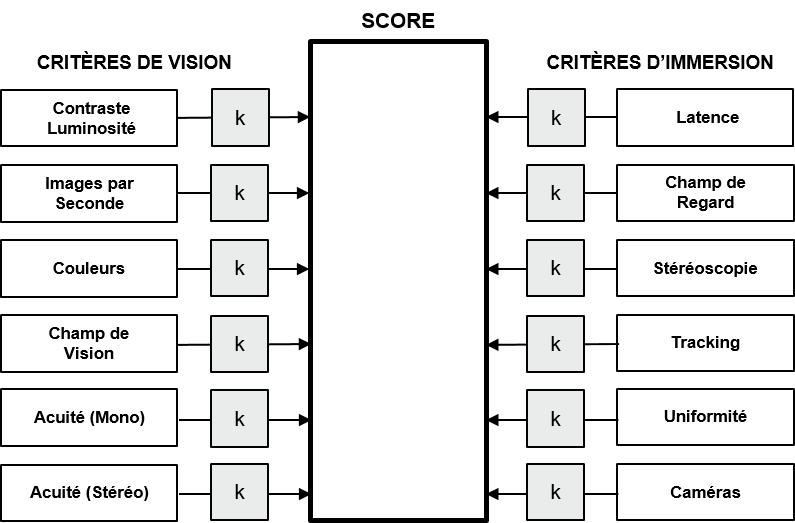
\includegraphics[scale=1]{Figures/ScoreRealismeMini}
		\caption{Rappel de la modélisation du score de réalisme.}
		\label{fig:score_realisme_mini}
	\end{figure}
	
	\subsection*{Résultats expérimentaux}
	\par Dans le cadre de la thèse, on a réalisé trois expérimentations: la validation d'un modèle de performance visuelle pour le critère de contraste et luminance, la mesure de performance pour le critère de latence et la comparaison entre les notations subjectives des critères du modèle par des sujets et les notes objectives données par notre modèle. Cette dernière, de moindre ampleur par rapport aux autres, dégage néanmoins quelques tendances. La pondération des critères de champ de vision et de champ de regard est très dépendante de l'application: dans le cas de la conduite, l'utilisation du champ de regard est quasi-nulle et les sujets ne font pas la différence entre les deux champs. Également, l'appréciation de la quotité de couleur semble sur-évaluée par habitude. Enfin, les femmes font preuve de plus de sévérité dans leur notation que les hommes.
	
	\par Pour l'expérimentation sur le critère de contraste et de luminance, on a cherché à traduire une expérimentation en Réalité Virtuelle, afin de déterminer si le modèle de performance visuelle mis en jeu était utilisable dans notre domaine. Ce modèle prédit des conditions de luminance et de contraste en dessous desquelles le système visuel humain n'est pas capable de distinguer ce qu'on lui demande, et des conditions au dessus desquelles la performance de détection de l'œil n'augmente plus. Il permet ainsi de déterminer la plage dans laquelle un moyen immersif devrait se situer. Nos résultats théoriques semblent se comporter de manière radicalement différente par rapport aux prévisions du modèle, tout en montrant une corrélation statistique. On montre que le modèle de performance visuelle est utilisable, sous réserve de l'inclusion d'un facteur prenant en compte les spécificités de la Réalité Virtuelle. Pour l'application à notre critère de contraste et luminance, on revient toutefois à préconiser une technique utilisant les fonctions de sensibilité au contraste et la découpe en fréquence spatiale des tâches classique de vision en immersif.
	
	\par Enfin, l'expérimentation sur la latence est quant à elle une comparaison entre deux systèmes et à différents niveaux de latence dans chaque système, de la performance de sujets à réaliser une tâche écologique. Les sujets devaient viser une série de cibles dans un véhicule modélisé en 3D, en maximisant leur précision par rapport au centre de la cible et leur vitesse de réalisation. On montre notamment que la performance se dégrade de manière non continue sous l'influence de la latence, tandis que le mal du simulateur est lui linéairement affecté. De même, le changement de système (de CAVE à casque) améliore la performance des sujets mais au détriment de leur expérience utilisateur: on met en cause la nature des mouvements impliqués pour la réalisation de la tâche demandée ainsi que le conflit visuo-vestibulaire.

	\subsection*{Travaux futurs}
	\par Si on présente une modélisation cohérente, il reste néanmoins des axes de travail et des propositions à améliorer ; le temps imparti pour la thèse ne nous ayant pas permis de tout traiter. Tout d'abord, bien que l'on ait eu des avancées concrètes pour le critère de contraste et luminance, nous ne sommes pas encore en mesure de pouvoir déterminer pratiquement son score. Par conséquent, le critère d'uniformité est encore à l'état d'embryon, étant intrinsèquement lié au contraste et à la luminance. On présente et on initie la suite des travaux sur le critère de contraste et de luminance avec l'utilisation des fréquences spatiales et des fonctions de contraste.
	
	\par D'autres critères cependant, tels que la quotité de couleur, la stéréoscopie et le tracking se sont vus attribuer une fonction de notation (linéaire ou binaire) que l'on juge insuffisante à terme ; ces notations sont fonctionnelles mais doivent être raffinées. On a présenté, par exemple dans le cas de la stéréoscopie, une piste d'amélioration de la fonction de notation, basée sur la technologie utilisée.
	
	\par La plus grande partie de futurs travaux reste la pondération du modèle. Si on propose des ordres de grandeur, il sera nécessaire, dans un second temps, d'avancer des propositions chiffrées, amenant plus de finesse pour départager les critères. Ces pondérations chiffrées seront très dépendantes du cas d'utilisation et permettront de prendre en compte certains scénarios spécifiques (comme la haute vitesse par exemple).
	
	\par Enfin, on peut également envisager une ouverture du score à d'autres types de systèmes, comme par exemple les systèmes de Réalité Augmentée qui apparaissent de plus en plus sur le marché. De même, le modèle pourrait être étoffé avec l'inclusion d'autres paradigmes qui composent l'expérience utilisateur: la présence, l'immersion, le confort, etc.

\section*{Application du score de réalisme}
\par Si la thèse a pour l'instant eu une application soit théorique, soit pratique mais au service de la théorie, il manque encore une application purement pratique de notre modèle de score. Or, on est désormais globalement en mesure d'appliquer notre modèle de score de réalisme visuel, à l'exception de deux critères intrinsèquement liés (critère de contraste et luminance, critère d'uniformité). On sélectionne des moyens immersifs présents chez Renault et on leur applique, sur chacun de leurs critères, les fonctions de notation déployées au cours de la thèse. Pour les critères non-aboutis, on utilise des estimations guidées par la littérature, à défaut de pouvoir les noter directement. De même, pour la pondération, on applique un coefficient uniforme de $2$ pour les critères <<~forts~>> et de $1$ pour les critères <<~faibles~>>. On sélectionne les systèmes suivants: deux CAVEs de chez Renault (nommés IRIS et P3I), un casque de Réalité Virtuelle grand public mais utilisé fréquemment dans l'industrie (HTC Vive) et un casque de Réalité Augmentée (Hololens). Techniquement, notre modèle de score n'est pas conçu pour une application en Réalité Augmentée, mais il peut être intéressant d'en tester les limites sur de tels dispositifs. Les résultats généraux de notation sont représentés en Fig. \ref{fig:resultats_score_application}.

\begin{figure}[h]
	\centering
	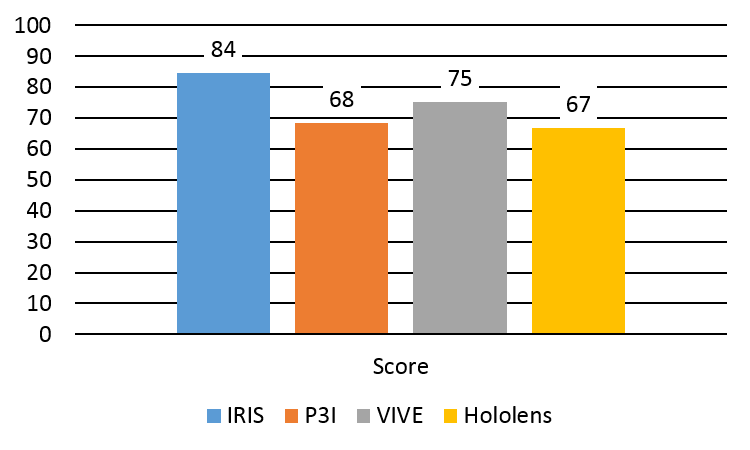
\includegraphics[scale=1]{Figures/ResultatsScoreApplication}
	\caption{Score de réalisme pour les quatre systèmes testés.}
	\label{fig:resultats_score_application}
\end{figure}

\par IRIS est un dispositif de type CAVE et possède 5 faces de $3~m$ d'arête. Il est le fleuron des technologies d'affichage immersif chez Renault. L'image de chaque face est affichée à l'aide de deux projecteurs 4K haute luminosité fonctionnant à $120~Hz$. Ces caractéristiques hors-norme permettent à IRIS d'avoir d'excellente notes que ce soit pour le contraste (80), le champ de vision (100), les acuités (98 et 67). Tous les calculs nécessitants la position de l'utilisateur sont fait par rapport à la position usuelle d'utilisation, c'est à dire à $1.30~m$ de la face avant, centré en largeur et avec une hauteur de tête à $1~m$ du sol. La latence moyenne est mesurée autour de $80~ms$. Toutes les notes d'IRIS sont résumées en Fig. \ref{fig:radar_score_iris}.

\begin{figure}[h]
	\centering
	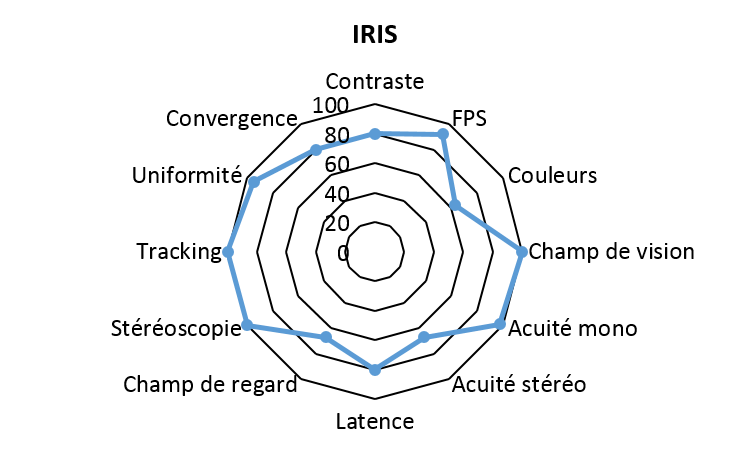
\includegraphics[scale=1]{Figures/RadarScoreIRIS}
	\caption{Diagramme radar des critères du score pour IRIS.}
	\label{fig:radar_score_iris}
\end{figure}

\par P3I est également un dispositif de type CAVE, que l'on connait bien car il a servi à la réalisation de nos expérimentations. On a donc déjà présenté ses caractéristiques principales, que ce soit en taille, résolution ou latence. Pour les calculs de champs et d'acuité on se place dans les mêmes conditions que pour IRIS, c'est à dire à $1.30~m$ de la face avant, centré en largeur et avec une hauteur de tête à $1~m$ du sol. Les notes de P3I pour les différents critères du modèle sont synthétisées en Fig. \ref{fig:radar_score_p3i}.

\begin{figure}[h]
	\centering
	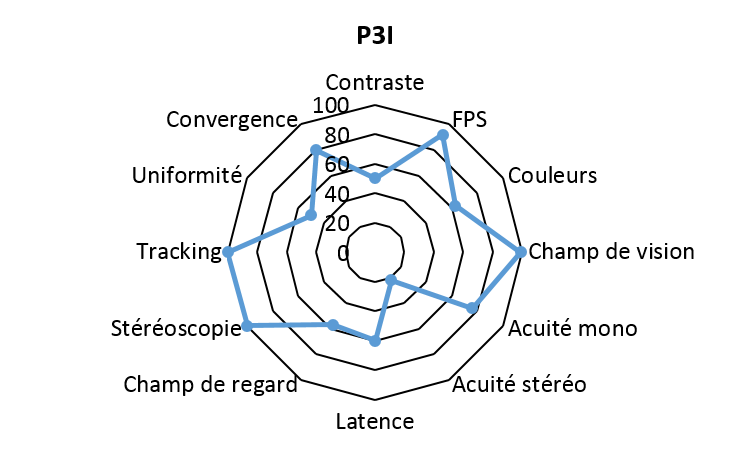
\includegraphics[scale=1]{Figures/RadarScoreP3I}
	\caption{Diagramme radar des critères du score pour P3I.}
	\label{fig:radar_score_p3i}
\end{figure}

\par On s'intéresse ensuite à un classique des casque de Réalité Virtuelle grand public mais largement présent dans le paysage industriel de la VR: le HTC Vive. Il possède un champ de vision horizontal de 110 degrés pour un écran de 3.6 pouces. Si son champ est donc légèrement plus petit que dans les solutions de type CAVE, il bénéficie néanmoins d'un champ de regard total. De manière analogue à l'Oculus Rift que l'on a utilisé pour notre expérimentation, le Vive fonctionne avec un taux de rafraichissement de $90~Hz$ et une latence mesurée d'environ $45~ms$. On retrouve le détail des notes du Vive en Fig. \ref{fig:radar_score_vive}.

\begin{figure}[h]
	\centering
	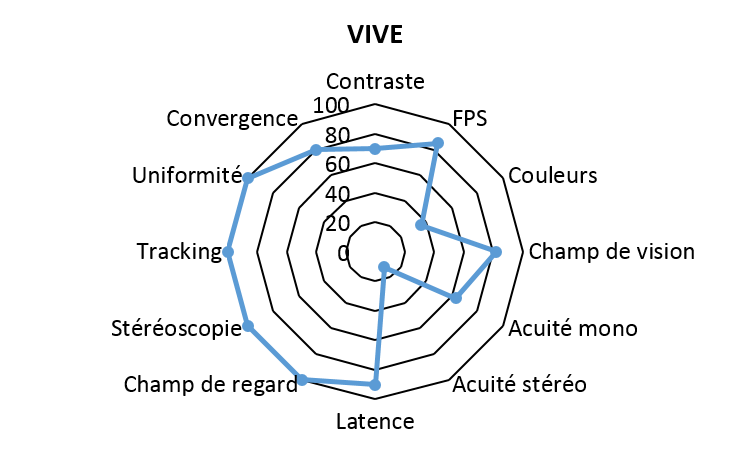
\includegraphics[scale=1]{Figures/RadarScoreVIVE}
	\caption{Diagramme radar des critères du score pour le casque VIVE.}
	\label{fig:radar_score_vive}
\end{figure}

\par Enfin, on applique notre modèle de score à l'Hololens de Microsoft, avec la particularité que ce dernier est un casque de Réalité Augmentée et non pas de Réalité Virtuelle. Il possède un champ de vision très réduit (30 par 17.5 degrés) pour une résolution assez faible (720p), ce qui explique ses notes assez faibles dans la partie indices de vision. C'est ici une limite de notre score de réalisme lorsqu'on l'applique à un système de RA: en réalité, le champ de vision est maximal car le casque ne fait que rajouter des informations sur la vision naturelle ; mais notre modèle juge la partie affichage seulement car celle-ci représente l'intégralité de la vision en Réalité Virtuelle. Néanmoins, le score est rattrapé par la partie indices d'immersion car le casque possède les mêmes qualités que ses homologues de Réalité Virtuelle: la stéréoscopie, une forme de tracking et surtout un champ de regard maximal avec la capacité d'orienter la tête dans n'importe quelle direction. Toutes ses notes sont résumées en Fig. \ref{fig:radar_score_hololens}.

\begin{figure}[h]
	\centering
	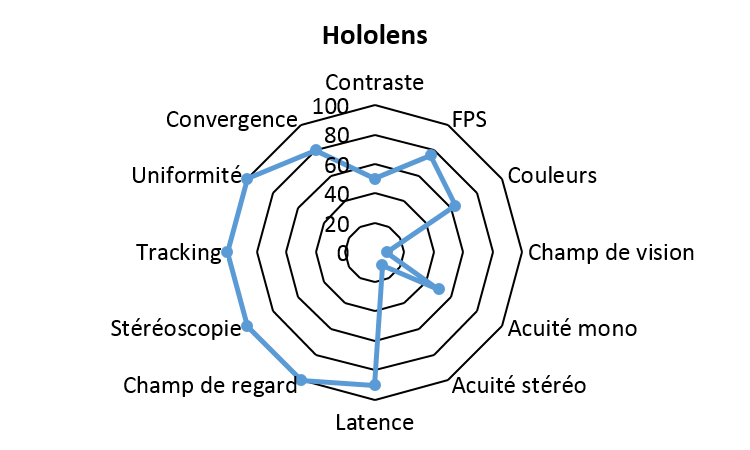
\includegraphics[scale=1]{Figures/RadarScoreHololens}
	\caption{Diagramme radar des critères du score pour le casque Hololens.}
	\label{fig:radar_score_hololens}
\end{figure}

\par Pour conclure, on remarque déjà que la hiérarchie des notes est cohérente avec notre ressenti d'utilisateur. On note également que les indices d'immersion (la partie gauche des diagrammes radar) sont en moyenne très bien notés: la différence se fait donc plutôt au niveau des indices de vision (partie droite des diagrammes radar), zone où les CAVEs sont globalement meilleurs. D'un point de vue purement stimulation visuelle, les CAVEs semblent donc plus recommandés. Néanmoins, d'autres critères interviennent aussi dans le choix d'un système (portabilité, coût, ...) et on ne doit donc pas se limiter aux indices visuels seuls. Cela nous mène à décrire des cas concrets d'utilisation du score de réalisme.

\section*{Perspectives d'utilisation}
\par Pour terminer ce manuscrit, on propose de présenter des idées concrètes d'utilisation de notre score de réalisme. Le premier usage étant évidemment celui de l'aide à la conception ou à la mise à jour des systèmes immersifs. Lorsque que l'on doit par exemple améliorer les caractéristiques d'un système de RV, les critères disposant déjà d'une bonne note ne seront pas à traiter en premier. De même, une partie du système ayant atteint le score maximal, ne nécessite à priori pas d'amélioration, à moins que cette dernière ait un effet direct sur un autre critère.

\par On peut ensuite imaginer un usage visant à déterminer la lisibilité dans un simulateur: en pondérant tous les critères liés à cette tâche (acuités, contraste et luminance, fluidité en cas de haute vitesse) et en réglant la pondération des critères moins inutiles à 0. On pourra alors estimer quel moyen immersif est le plus adapté à des expérimentations impliquant de petits détails au loin comme la lecture en amont de panneaux d'autoroute (destination, limitations de vitesse, ...).

\par Enfin, il existe depuis 2016 une initiative permettant de mettre en location, à d'autres professionnels, ses systèmes immersifs: VR-BNB. Les entreprises (ou laboratoires) créent alors une page décrivant le système qu'elles mettent à disposition: on peut imaginer intégrer sur cette page, ou dans les critères de recherche, le score de réalisme dudit système, en pondération globale ou pondéré dans un cas d'utilisation spécifique. Les futurs utilisateurs auraient alors plus d'indications sur la capacité du système qu'ils envisagent de louer à répondre à leurs besoins expérimentaux.